\documentclass[twoside]{book}

% Packages required by doxygen
\usepackage{fixltx2e}
\usepackage{calc}
\usepackage{doxygen}
\usepackage[export]{adjustbox} % also loads graphicx
\usepackage{graphicx}
\usepackage[utf8]{inputenc}
\usepackage{makeidx}
\usepackage{multicol}
\usepackage{multirow}
\PassOptionsToPackage{warn}{textcomp}
\usepackage{textcomp}
\usepackage[nointegrals]{wasysym}
\usepackage[table]{xcolor}

% Font selection
\usepackage[T1]{fontenc}
\usepackage[scaled=.90]{helvet}
\usepackage{courier}
\usepackage{amssymb}
\usepackage{sectsty}
\renewcommand{\familydefault}{\sfdefault}
\allsectionsfont{%
  \fontseries{bc}\selectfont%
  \color{darkgray}%
}
\renewcommand{\DoxyLabelFont}{%
  \fontseries{bc}\selectfont%
  \color{darkgray}%
}
\newcommand{\+}{\discretionary{\mbox{\scriptsize$\hookleftarrow$}}{}{}}

% Page & text layout
\usepackage{geometry}
\geometry{%
  a4paper,%
  top=2.5cm,%
  bottom=2.5cm,%
  left=2.5cm,%
  right=2.5cm%
}
\tolerance=750
\hfuzz=15pt
\hbadness=750
\setlength{\emergencystretch}{15pt}
\setlength{\parindent}{0cm}
\setlength{\parskip}{0.2cm}
\makeatletter
\renewcommand{\paragraph}{%
  \@startsection{paragraph}{4}{0ex}{-1.0ex}{1.0ex}{%
    \normalfont\normalsize\bfseries\SS@parafont%
  }%
}
\renewcommand{\subparagraph}{%
  \@startsection{subparagraph}{5}{0ex}{-1.0ex}{1.0ex}{%
    \normalfont\normalsize\bfseries\SS@subparafont%
  }%
}
\makeatother

% Headers & footers
\usepackage{fancyhdr}
\pagestyle{fancyplain}
\fancyhead[LE]{\fancyplain{}{\bfseries\thepage}}
\fancyhead[CE]{\fancyplain{}{}}
\fancyhead[RE]{\fancyplain{}{\bfseries\leftmark}}
\fancyhead[LO]{\fancyplain{}{\bfseries\rightmark}}
\fancyhead[CO]{\fancyplain{}{}}
\fancyhead[RO]{\fancyplain{}{\bfseries\thepage}}
\fancyfoot[LE]{\fancyplain{}{}}
\fancyfoot[CE]{\fancyplain{}{}}
\fancyfoot[RE]{\fancyplain{}{\bfseries\scriptsize Generated by Doxygen }}
\fancyfoot[LO]{\fancyplain{}{\bfseries\scriptsize Generated by Doxygen }}
\fancyfoot[CO]{\fancyplain{}{}}
\fancyfoot[RO]{\fancyplain{}{}}
\renewcommand{\footrulewidth}{0.4pt}
\renewcommand{\chaptermark}[1]{%
  \markboth{#1}{}%
}
\renewcommand{\sectionmark}[1]{%
  \markright{\thesection\ #1}%
}

% Indices & bibliography
\usepackage{natbib}
\usepackage[titles]{tocloft}
\setcounter{tocdepth}{3}
\setcounter{secnumdepth}{5}
\makeindex

% Hyperlinks (required, but should be loaded last)
\usepackage{ifpdf}
\ifpdf
  \usepackage[pdftex,pagebackref=true]{hyperref}
\else
  \usepackage[ps2pdf,pagebackref=true]{hyperref}
\fi
\hypersetup{%
  colorlinks=true,%
  linkcolor=blue,%
  citecolor=blue,%
  unicode%
}

% Custom commands
\newcommand{\clearemptydoublepage}{%
  \newpage{\pagestyle{empty}\cleardoublepage}%
}

\usepackage{caption}
\captionsetup{labelsep=space,justification=centering,font={bf},singlelinecheck=off,skip=4pt,position=top}

%===== C O N T E N T S =====

\begin{document}

% Titlepage & ToC
\hypersetup{pageanchor=false,
             bookmarks=true,
             bookmarksnumbered=true,
             pdfencoding=unicode
            }
\pagenumbering{roman}
\begin{titlepage}
\vspace*{7cm}
\begin{center}%
{\Large Gym Prototype }\\
\vspace*{1cm}
{\large Generated by Doxygen 1.8.11}\\
\end{center}
\end{titlepage}
\clearemptydoublepage
\tableofcontents
\clearemptydoublepage
\pagenumbering{arabic}
\hypersetup{pageanchor=true}

%--- Begin generated contents ---
\chapter{R\+E\+A\+D\+ME}
\label{md_README}
\hypertarget{md_README}{}
\#\+S\+E\+NG 330

\subsection*{Install}


\begin{DoxyEnumerate}
\item Run make ``` make ```
\item Run the resulting executable \textquotesingle{}prototype\textquotesingle{} ``` ./prototype ``` 
\end{DoxyEnumerate}
\chapter{Hierarchical Index}
\section{Class Hierarchy}
This inheritance list is sorted roughly, but not completely, alphabetically\+:\begin{DoxyCompactList}
\item \contentsline{section}{Factory}{\pageref{class_factory}}{}
\item \contentsline{section}{Gym\+Item}{\pageref{class_gym_item}}{}
\begin{DoxyCompactList}
\item \contentsline{section}{Stationary\+Bike}{\pageref{class_stationary_bike}}{}
\item \contentsline{section}{Treadmill}{\pageref{class_treadmill}}{}
\end{DoxyCompactList}
\end{DoxyCompactList}

\chapter{Class Index}
\section{Class List}
Here are the classes, structs, unions and interfaces with brief descriptions\+:\begin{DoxyCompactList}
\item\contentsline{section}{\hyperlink{class_factory}{Factory} }{\pageref{class_factory}}{}
\item\contentsline{section}{\hyperlink{class_gym_item}{Gym\+Item} }{\pageref{class_gym_item}}{}
\item\contentsline{section}{\hyperlink{class_stationary_bike}{Stationary\+Bike} }{\pageref{class_stationary_bike}}{}
\item\contentsline{section}{\hyperlink{class_treadmill}{Treadmill} }{\pageref{class_treadmill}}{}
\end{DoxyCompactList}

\chapter{Class Documentation}
\hypertarget{class_factory}{}\section{Factory Class Reference}
\label{class_factory}\index{Factory@{Factory}}
\subsection*{Static Public Member Functions}
\begin{DoxyCompactItemize}
\item 
static \hyperlink{class_gym_item}{Gym\+Item} $\ast$ {\bfseries make\+\_\+machine} (int choice)\hypertarget{class_factory_aad54b69d2fbeb1a61a8519be07015cdc}{}\label{class_factory_aad54b69d2fbeb1a61a8519be07015cdc}

\end{DoxyCompactItemize}


The documentation for this class was generated from the following file\+:\begin{DoxyCompactItemize}
\item 
prototype.\+cpp\end{DoxyCompactItemize}

\hypertarget{class_gym_item}{}\section{Gym\+Item Class Reference}
\label{class_gym_item}\index{Gym\+Item@{Gym\+Item}}
Inheritance diagram for Gym\+Item\+:\begin{figure}[H]
\begin{center}
\leavevmode
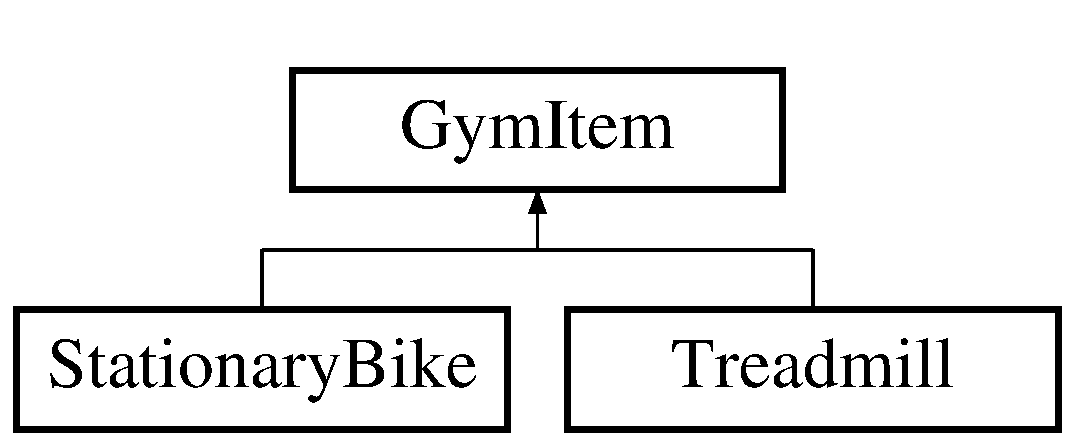
\includegraphics[height=2.000000cm]{class_gym_item}
\end{center}
\end{figure}
\subsection*{Public Member Functions}
\begin{DoxyCompactItemize}
\item 
virtual \hyperlink{class_gym_item}{Gym\+Item} $\ast$ {\bfseries clone} ()=0\hypertarget{class_gym_item_a2c0c7b444e2c64288c91bfa14ac48c8e}{}\label{class_gym_item_a2c0c7b444e2c64288c91bfa14ac48c8e}

\item 
virtual void {\bfseries start\+\_\+machine} ()=0\hypertarget{class_gym_item_ad449e15b73f9aa2f1fea30ee63ad538b}{}\label{class_gym_item_ad449e15b73f9aa2f1fea30ee63ad538b}

\end{DoxyCompactItemize}


The documentation for this class was generated from the following file\+:\begin{DoxyCompactItemize}
\item 
prototype.\+cpp\end{DoxyCompactItemize}

\hypertarget{class_stationary_bike}{}\section{Stationary\+Bike Class Reference}
\label{class_stationary_bike}\index{Stationary\+Bike@{Stationary\+Bike}}
Inheritance diagram for Stationary\+Bike\+:\begin{figure}[H]
\begin{center}
\leavevmode
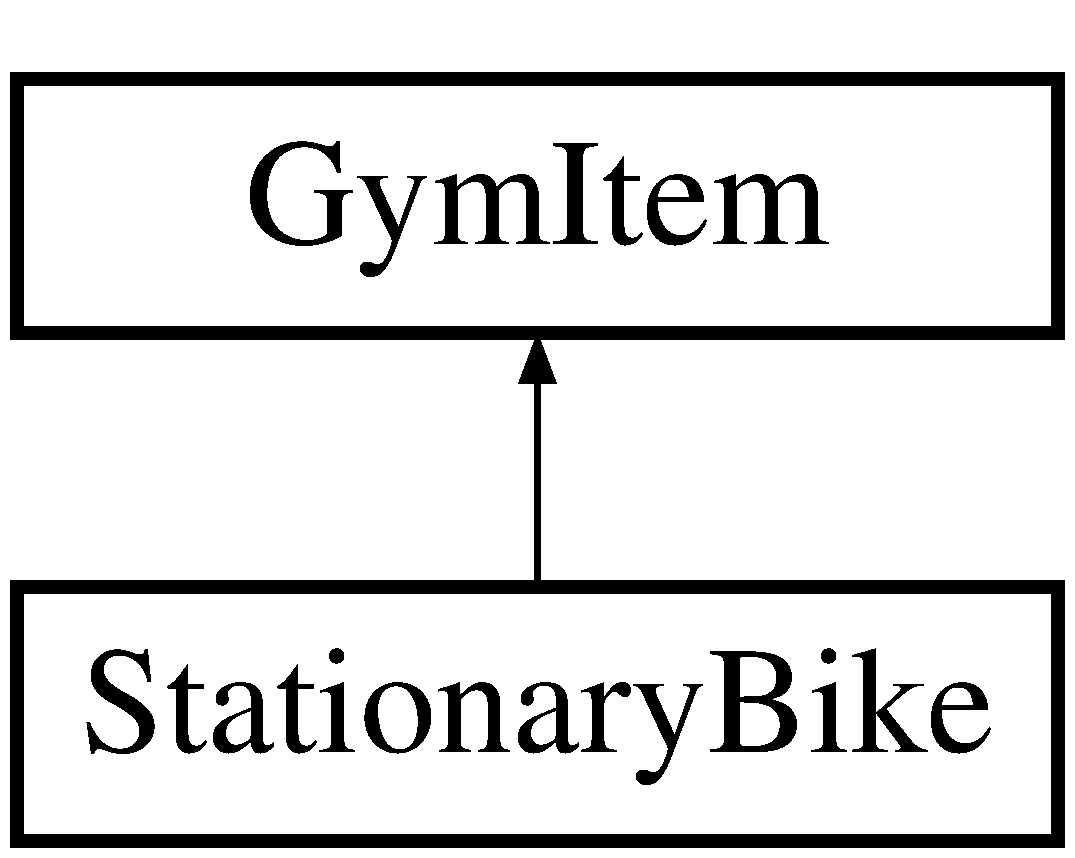
\includegraphics[height=2.000000cm]{class_stationary_bike}
\end{center}
\end{figure}
\subsection*{Public Member Functions}
\begin{DoxyCompactItemize}
\item 
\hyperlink{class_gym_item}{Gym\+Item} $\ast$ {\bfseries clone} ()\hypertarget{class_stationary_bike_a1bc68c2ac559ec24cfd2829005d38c39}{}\label{class_stationary_bike_a1bc68c2ac559ec24cfd2829005d38c39}

\item 
void {\bfseries start\+\_\+machine} ()\hypertarget{class_stationary_bike_a5aef9ee065dbbe58d48613443cf651cb}{}\label{class_stationary_bike_a5aef9ee065dbbe58d48613443cf651cb}

\end{DoxyCompactItemize}


The documentation for this class was generated from the following file\+:\begin{DoxyCompactItemize}
\item 
prototype.\+cpp\end{DoxyCompactItemize}

\hypertarget{class_treadmill}{}\section{Treadmill Class Reference}
\label{class_treadmill}\index{Treadmill@{Treadmill}}
Inheritance diagram for Treadmill\+:\begin{figure}[H]
\begin{center}
\leavevmode
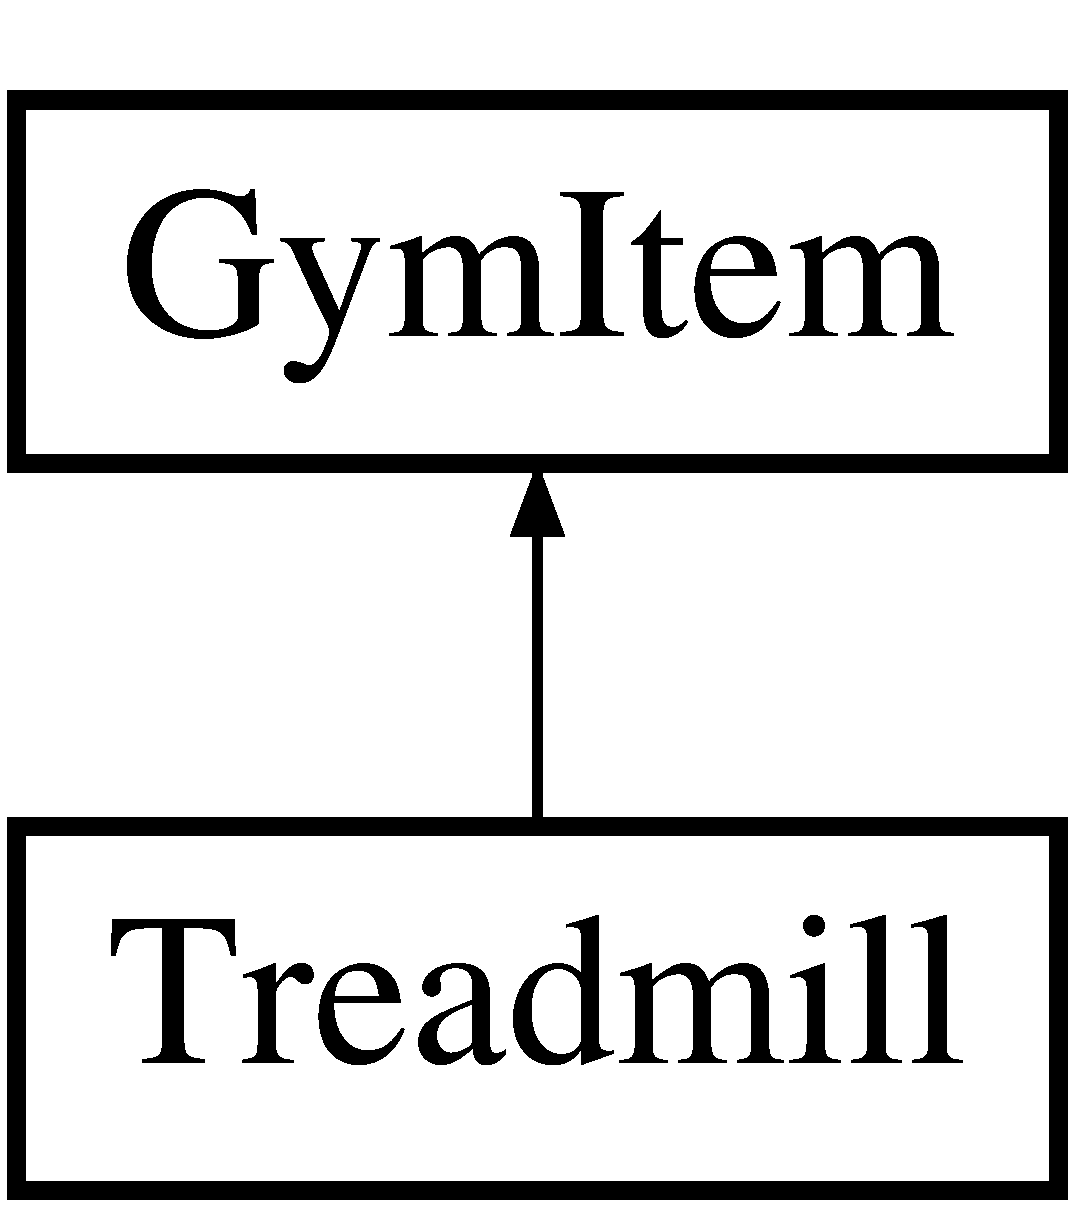
\includegraphics[height=2.000000cm]{class_treadmill}
\end{center}
\end{figure}
\subsection*{Public Member Functions}
\begin{DoxyCompactItemize}
\item 
\hyperlink{class_gym_item}{Gym\+Item} $\ast$ {\bfseries clone} ()\hypertarget{class_treadmill_ae44ece9910774bfe1161e6831c893fdd}{}\label{class_treadmill_ae44ece9910774bfe1161e6831c893fdd}

\item 
void {\bfseries start\+\_\+machine} ()\hypertarget{class_treadmill_aaa9004a3be6ca94939c901a2d1e48d84}{}\label{class_treadmill_aaa9004a3be6ca94939c901a2d1e48d84}

\end{DoxyCompactItemize}


The documentation for this class was generated from the following file\+:\begin{DoxyCompactItemize}
\item 
prototype.\+cpp\end{DoxyCompactItemize}

%--- End generated contents ---

% Index
\backmatter
\newpage
\phantomsection
\clearemptydoublepage
\addcontentsline{toc}{chapter}{Index}
\printindex

\end{document}
